\section{Theoretical Analysis}
\label{sec:analysis}

For the theoretical simulation, we used the ideal diode model for the full-wave bridge rectifier, obtaining the absolute value of the initial signal.

For the limiter circuit associated with a first-order low-pass filter, we performed fourier analysis on the previously obtained signal, in order to use phasors to solve for the voltage on the capacitor.
The vON diode model was used in this stage, such that any voltage above n*vON (n being the number of diodes in this part of the circuit) was limited.

The envelope detector was analysed with the tOFF method, with its value being determined by the below equation:

\begin{equation}
	\frac{dVs}{dt}=-\frac{Vs}{RC}
\end{equation}

After time tOFF the output voltage of this part of the circuit was modeled using an exponecial, until it crossed the input voltage once more.
We see the rectified and limited voltage, as well as the output of the envelope detector below:

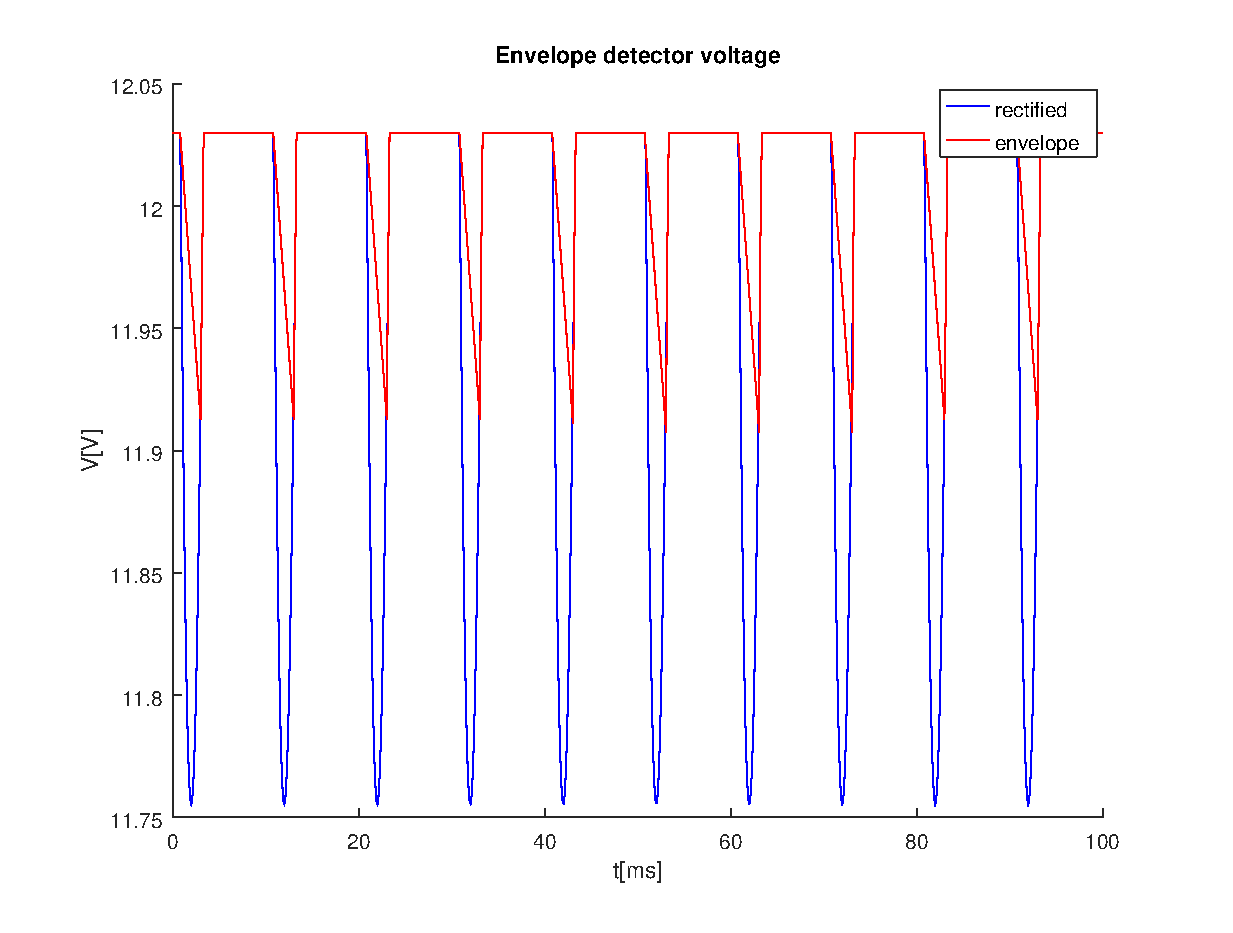
\includegraphics[width=1\linewidth]{venvelope.eps}

For the low-pass filter at the end, we used the Euler method to solve the differencial equation for an RC circuit, thus obtaining the final output voltage:

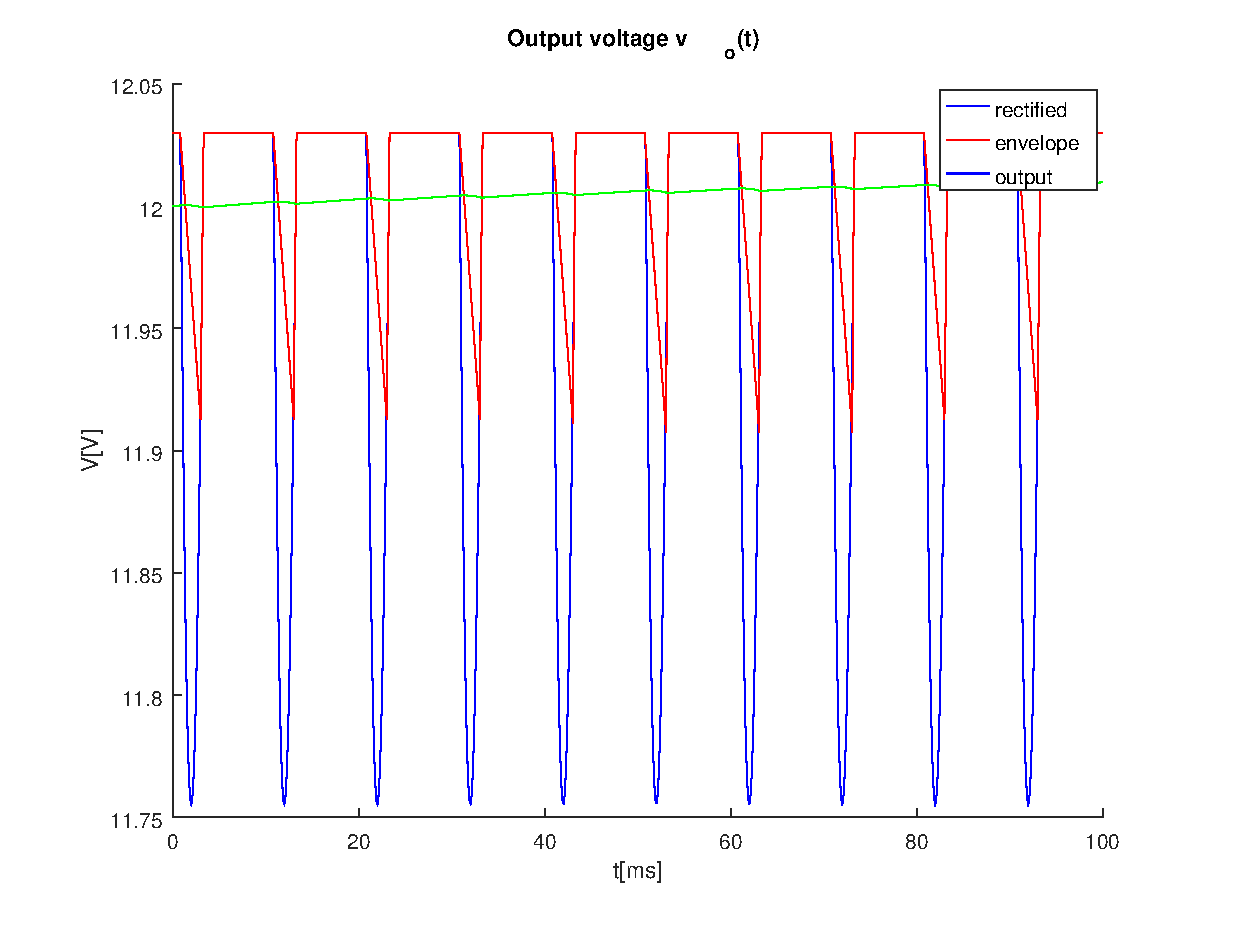
\includegraphics[width=1\linewidth]{voutput.eps}

We can also see the circuit stabilizing from time t=0:

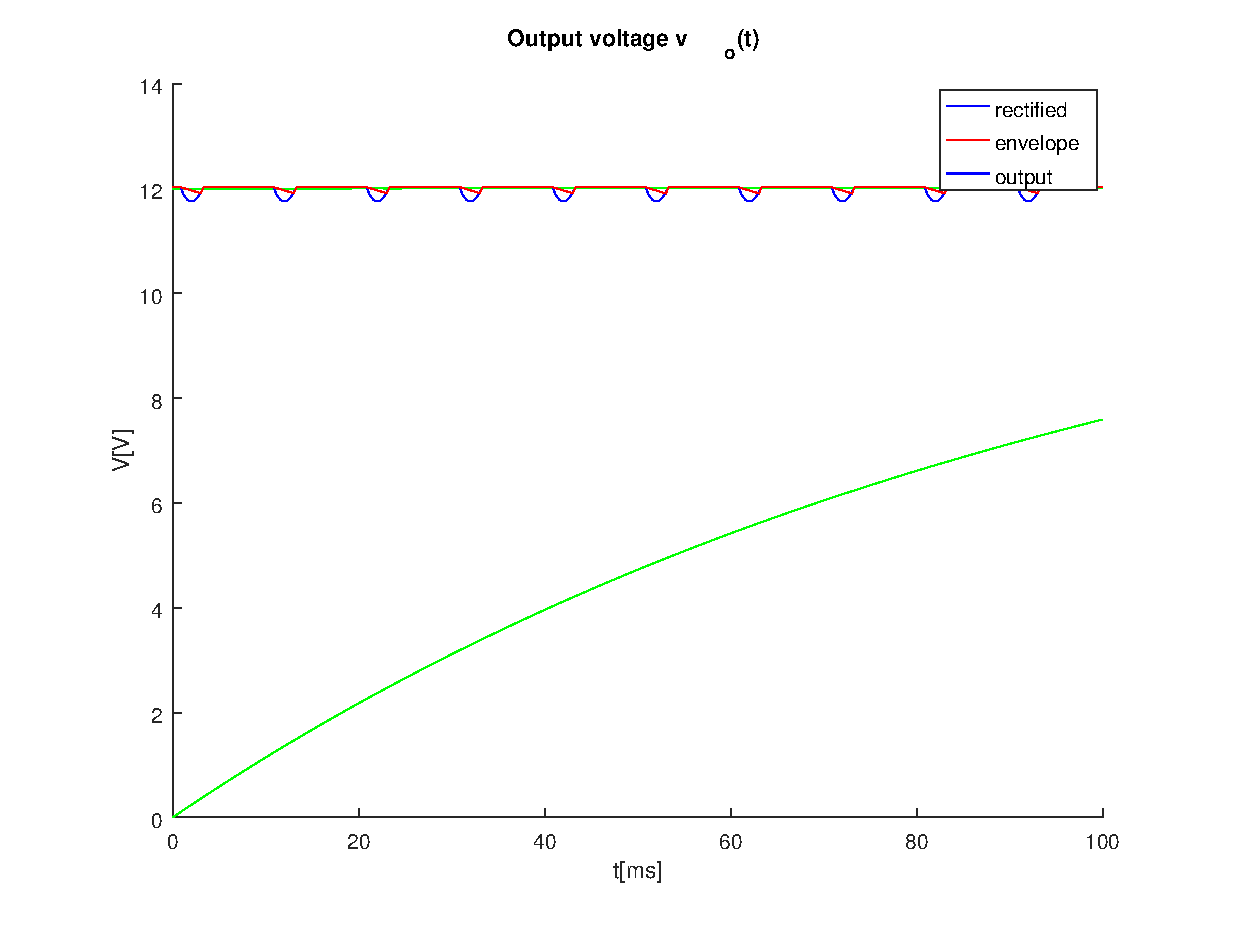
\includegraphics[width=1\linewidth]{voutput_init.eps}


The values of the ripple and average voltage were calculated and are $0.010181$
and $12.005305$ respectively

